% !Mode:: "TeX:UTF-8"
% !TEX program  = pdflatex
\documentclass{article}
\usepackage[ruled,vlined,linesnumbered]{algorithm2e}
\usepackage{algpseudocode}
\usepackage{amsmath}
\usepackage{amsthm}
\usepackage{graphicx}
\usepackage{subfigure}
\usepackage{float}
\usepackage{amssymb}
\usepackage{amsfonts}
\usepackage{mathrsfs}
\usepackage{pdfpages}
\usepackage{epsfig}
\usepackage{graphicx}
\usepackage{arydshln}
\usepackage{verbatim}
\usepackage{subfigure}
\usepackage{enumerate}
\usepackage{rotating}
\usepackage{threeparttable}
\usepackage{caption}
\usepackage{epsfig}
\usepackage{cite}
\usepackage{tikz}
\usetikzlibrary{shapes}
\usetikzlibrary{shapes.geometric}
\usepackage{geometry}
\geometry{a4paper, top=2.54cm, bottom=2.54cm, left=3.18cm, right=3.18cm}
\theoremstyle{definition}
\newtheorem{prob}{Problem}
\newtheorem{ans}{Answer}
\usepackage[colorlinks,linkcolor=black]{hyperref}
\linespread{1.2}
\begin{document}
	
	\section*{\LARGE [Homework 2] Finite Markov Chains, Coupling}
	\section*{\large Kailing Wang 521030910356}
	
	\section*{Problem 1 (Optimal Coupling)}
	First recall the definition of $D_{\operatorname{TV}}(\mu, \nu)$:
	$$
	\begin{aligned}
		D_{\operatorname{TV}}(\mu, \nu) & = \frac{1}{2}\underset{i \in \Omega}{\sum}|\mu(i)-\nu(i)|\\
		& = \underset{\substack{ i \in \Omega, \\ \mu(i)\geq\nu(i)}}{\sum}\left(\mu(i)-\nu(i)\right) = \underset{\substack{ i \in \Omega, \\ \mu(i)<\nu(i)}}{\sum}\left(\nu(i)-\mu(i)\right)
	\end{aligned}	
	$$
	From the mathematical form, we can see that if we construct a coupling $\omega$ that satisfies
	\begin{equation}
		\mathbf{Pr}_{(X,Y)\sim\omega}[X=Y=i]=\omega(i, i)=\min\{\mu(i), \nu(i)\}
		\label{r1}
	\end{equation}
	We get 
	$$
	\begin{aligned}
		\mathbf{Pr}_{(X,Y)\sim\omega}[X\neq Y] & = 1-\underset{i \in \Omega}{\sum}\mathbf{Pr}_{(X,Y)\sim\omega}[X = Y = i] \\ 
		& = \underset{i \in \Omega}{\sum}\mu(i)-\underset{i \in \Omega}{\sum}\min\{\mu(i), \nu(i)\} \\
		& = \underset{\substack{ i \in \Omega, \\ \mu(i)\geq\nu(i)}}{\sum}\left(\mu(i)-\nu(i)\right)
	\end{aligned}
	$$
	Then we only have to prove that using equation (\ref{r1}) we can construct a legal coupling method. We want to have a closed form solution for $\omega(i,j)\text{ when } i\neq j$, 
	\begin{equation}
		\omega(i,j) = \frac{\max \{\mu(i)-\nu(i), 0\} \cdot \max \{\nu(j)-\mu(j), 0\}}{D_{\operatorname{TV}}(\mu, \nu)}
	\end{equation}
	\noindent I modified my expression based on lecture notes from MIT\cite{mit3}. This construction is legal for
	$$
	\begin{aligned}
		\sum_{j \in \Omega} \omega(i, j) & =\min \{\mu(i), \nu(i)\}+\sum_{\substack{j \in \Omega \\
				j \neq i}} \omega(x, y) \\
		& =\min \{\mu(i), \nu(i)\}+\max \{\mu(i)-\nu(i), 0\} \cdot \frac{\underset{\substack{j \in \Omega \\
					j \neq i}}{\sum} \max \{\nu(j)-\mu(j), 0\}}{D_{\operatorname{TV}}(\mu, \nu)} 
	\end{aligned}
	$$
	\begin{itemize}
		\item when $\mu(i)\geq\nu(i)$
		$$
		\begin{aligned}
			\sum_{j \in \Omega} \omega(i, j) & =\nu(i)+(\mu(i)-\nu(i)) \cdot \frac{\underset{\mu(j)<\nu(j)}{\sum}(\nu(j)-\mu(j))}{D_{\operatorname{TV}}(\mu, \nu)} \\
			& =\nu(i)+\mu(i)-\nu(i) \\
			& =\mu(i)
		\end{aligned}
		$$
		\item when $\mu(i)<\nu(i)$
		$$
		\begin{aligned}
			\sum_{j \in \Omega} \omega(i, j) & =\mu(i)+ 0 \cdot \frac{\underset{\substack{j \in \Omega \\
						j \neq i}}{\sum} \max \{\nu(j)-\mu(j), 0\}}{D_{\operatorname{TV}}(\mu, \nu)} \\
			& =\mu(i)
		\end{aligned}
		$$
		and it's similar to $\nu$.
	\end{itemize}
	
	\section*{Problem 2 (Total Variation Distance is Non-Increasing)}
	We denote two random variables $X_t\sim \mu_t, ~Y_t\sim \pi$. We can construct a coupling method by 
	\begin{itemize}
		\item $X_t$ and $Y_t$ move independently if they have not met each other.
		\item $X_t$ and $Y_t$ move together since they met.
	\end{itemize}
	This way, 
	\begin{equation}
		\Delta(t+1) = \frac{1}{2}\underset{i \in \Omega}{\sum}|\mu_{t+1}(i)-\pi(i)|\leq \mathbf{Pr}[X^{t+1}\neq Y^{t+1}]\leq \mathbf{Pr}[X^{t}\neq Y^{t}]
		\label{ueq1}
	\end{equation}
	In problem 1 we've proved that there exists a $\omega^*$ that satisfies 
	\begin{equation}
		\mathbf{Pr}_{(X^t,Y^t)\sim\omega^*}[X^t\neq Y^t] = D_{\operatorname{TV}}(\mu^t, \pi) = \Delta(t)
		\label{ueq2}
	\end{equation}
	Thus with equation \ref{ueq1} and \ref{ueq2} we get $\Delta(t+1)\leq\Delta(t)$. We use a coupling composed of the one in problem 1 and the one mentioned above. 
	
	\section*{Problem 3}
	To make a simple guess: HT is more likely to appear first because it is more `pointed'.
	
	\noindent To explicitly describe the process, I draw the state map of sequence with length 2. There are in total 4 possible sequences with uniform distribution initially. From each state, we can obtain two possible states depending on the results of the coin tossing. We denote the minimum time a pattern $X$ appears by $T_X$. 
	\begin{center}
		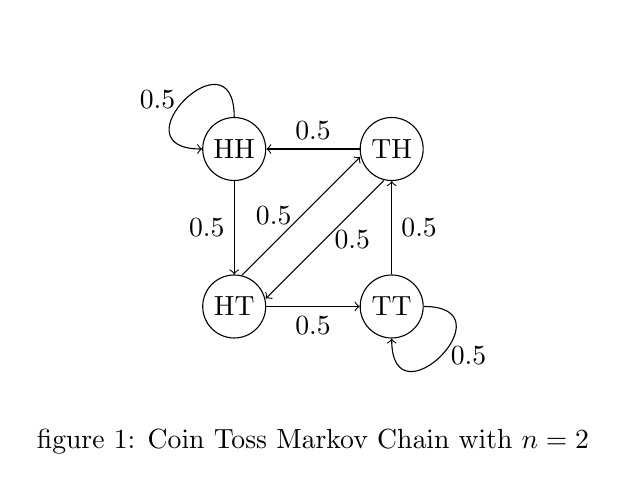
\begin{tikzpicture}
			[vertex/.style={circle, draw, inner sep=0pt, minimum size=8mm}]
			
			\node[vertex] (A) at (0,2) {HH};
			\node[vertex] (B) at (0,0) {HT};
			\node[vertex] (C) at (2,2) {TH};
			\node[vertex] (D) at (2,0) {TT};
			
			\draw[->] (A) to node[midway, left] {0.5} (B);
			\draw[->] (0.1,0.4) to node[midway, left] {0.5} (1.6,1.9);
			\draw[->] (B) to node[midway, below] {0.5} (D);
			\draw[->] (C) to node[midway, above] {0.5} (A);
			\draw[->] (1.9,1.6) to node[midway, right] {0.5} (0.4,0.1);
			\draw[->] (D) to node[midway, right] {0.5} (C);
			
			\draw[->] (A) to[out=90, in=180, looseness=5] node[midway, left] {0.5}(A);
			\draw[->] (D) to[out=0, in=270, looseness=5] node[midway, right] {0.5}(D);
			
			\node[above] at (1,-2) {figure 1: Coin Toss Markov Chain with $n=2$};
		\end{tikzpicture}
	\end{center}
	We denote the minimum time to form a pattern $Y$ from pattern $X$ by $T_{X\rightarrow Y}$. Suppose we start at pattern $HH$, then it takes 0 to reach $HH$. If we start at $HT$, we have $\frac{1}{2}$ chance to get $TH$ and then take $T_{TH\rightarrow HH}$ to get $HH$, and $\frac{1}{2}$ chance to get $TT$ and then take $T_{TT\rightarrow HH}$ to get $HH$. It's similar to getting started at $TH$ and $TT$. In total we have
	$$
	\left\{
	\begin{array}{l}
		T_{HH\rightarrow HH} = 0 \\
		T_{TH\rightarrow HH} = \frac{1}{2}(1+T_{HT\rightarrow HH}) + \frac{1}{2}(1+T_{HH\rightarrow HH}) = \frac{1}{2}T_{HT\rightarrow HH} + 1 \\
		T_{HT\rightarrow HH} = \frac{1}{2}(1+T_{TT\rightarrow HH}) + \frac{1}{2}(1+T_{TH\rightarrow HH}) = \frac{1}{2}T_{HT\rightarrow HH} + \frac{1}{2}T_{TH\rightarrow HH} + 1 \\
		T_{TT\rightarrow HH} = \frac{1}{2}(1+T_{TT\rightarrow HH}) + \frac{1}{2}(1+T_{TH\rightarrow HH}) = \frac{1}{2}T_{TT\rightarrow HH} + \frac{1}{2}T_{TH\rightarrow HH} + 1
	\end{array}
	\right.
	$$
	Consider the expectation, 
	$$
	\left\{
	\begin{array}{l}
		\mathbf E[T_{HH\rightarrow HH}] = 0 \\
		\mathbf E[T_{TH\rightarrow HH}] = \frac{1}{2}\mathbf E[T_{HT\rightarrow HH}] + 1 \\
		\mathbf E[T_{HT\rightarrow HH}] = \frac{1}{2}\mathbf E[T_{TT\rightarrow HH}] + \frac{1}{2}\mathbf E[T_{TH\rightarrow HH}] + 1 \\
		\mathbf E[T_{TT\rightarrow HH}] = \frac{1}{2}\mathbf E[T_{TT\rightarrow HH}] + \frac{1}{2}\mathbf E[T_{TH\rightarrow HH}] + 1
	\end{array}
	\right.
	$$
	solve the system of equations, we get
	$$
	\left\{
	\begin{array}{l}
		\mathbf E[T_{HH\rightarrow HH}] = 0 \\
		\mathbf E[T_{TH\rightarrow HH}] = 4 \\
		\mathbf E[T_{HT\rightarrow HH}] = 6 \\
		\mathbf E[T_{TT\rightarrow HH}] = 6
	\end{array}
	\right.
	$$
	Then $\mathbf E[T_1] = 2 + \frac{1}{4}(0+4+6+6) = 6$. Similarly, $\mathbf E[T_2] = 2 + \frac{1}{4}(2+2+0+4) = 4$. The constant 2 refers to the time to get a certain initial state.
	\begin{itemize}
		\item \textbf{bonus}: To generalize, for a pattern with length n, we can simply use a state map with $2^n$ initial state with uniform distribution. According to the state map we can list the system of equations and solve them alike.
	\end{itemize}
	
	\section*{Problem 4 (Path Coupling)}
	At first I didn't really understand this question. I guess the statement of the problem skips too much detail. In class we designed a coupling for two random variables $X$ and $Y$ from $\mu$ and $\pi$ respectively to show the mixing time can be bounded. However, here it says `$\mathbf{E}\left[d\left(X_{t+1}, Y_{t+1}\right) \mid\left(X_t, Y_t\right)\right] \leq(1-\alpha) \cdot d\left(X_t, Y_t\right) \text { for those }\left(X_t, Y_t\right) \text { with } d\left(X_t, Y_t\right)=1$', but in the coupling in class we had no such restrictions as $d\left(X_t, Y_t\right)=1$. I later refer to more notes\cite{washington, mit6} to find that $d\left(X_t, Y_t\right)=1$ is not required in the example in class. It's something else we claim when constructing path coupling for sample coloring. 
	
	\noindent Now we verify about the irreducible component and its stationary distribution. When we try to transform a proper coloring to another proper coloring transform the by changing their disagreeing vertices one by one, if we met a improper intermediate state, we undo the most recent recoloring and seek a legal color instead to recolor and skip this vertex for later. We only need $q\geq \Delta+2$ to ensure we can always find this replacement color. Repeat this process we can always reach the target state, and so this component is irreducible. Since we do not allow transition from a proper coloring to a improper one while improper coloring can move to a proper one, a improper coloring super-vertex has only out-degree but 0 in-degree. This indicates they are transient and have probability 0 in the stationary distribution. Thus the stationary distribution is still the uniform distribution on all proper coloring methods. 
	\begin{enumerate}[(1)]
		\item When we couple a pair of variables, we are actually making both decision depending on a same tossed coin. Now suppose we have coupled $(Z_0, Z_1)$ to get $(Z_0', Z_1')$, $Z_0'$ is obtained by $Z_0$ taking one step on the Markov chain. The step taken by $Z_1$ depends on the high dimensional coin (a dice, let's say) tossed by $Z_0$. As we go on to couple $(Z_i, Z_{i+1})$, we are still making decision on this coin, and thus if viewed independently, we can say that $z_0$ and $z_k$ moves independently. We claim $\left(X_{t+1}, Y_{t+1}\right)=\left(z_0, z_k\right) \text { is a legal coupling of }\left(X_t, Y_t\right)$. 
		
		\noindent Here there is a confusing point. In the Markov chain mentioned in class, we do not allow any transition to improper coloring. Here there exists a coupling (defined in the third question) that holds the same rule on the new state space (i.e. we do not allow transitions that cause more improper pairs). I suggest in the first two question we assume the coupling is given and is an abstract one that satisfies $\mathbf{E}\left[d\left(X_{t+1}, Y_{t+1}\right) \mid\left(X_t, Y_t\right)\right] \leq(1-\alpha) \cdot d\left(X_t, Y_t\right)$.
		
		\noindent [Additional] According to the explanation given in class, I decide to provide a more explicit solution. Now suppose we have a path with length 3, i.e. $Z_i$, $Z_{i+1}$ and $Z_{i+2}$. We have a legal couple for both pair with distance 1. Imagine we still have a coin here, and we already know the joint distribution. Suppose $Z_{k}'$ have $n_{k}$ possible destinations here. From the joint distribution we can write 
		\begin{equation}
			\mathbf{Pr}[Z_{i+1} = d_{i+1}(j)] = \overunderset{n_{i}}{k=1}{\sum}\mathbf{Pr}_{(Z_i, Z_{i+1})\sim \omega}[Z_{i+1} = d_{i+1}(j) \wedge Z_i = d_i(k)]
			\label{add1}
		\end{equation}		
		\begin{equation}
			\mathbf{Pr}[Z_{i+2} = d_{i+2}(j)] = \overunderset{n_{i+1}}{k=1}{\sum}\mathbf{Pr}_{(Z_{i+1}, Z_{i+2})\sim \omega}[Z_{i+2} = d_{i+2}(j) \wedge Z_{i+1} = d_{i+1}(k)]
			\label{add2}
		\end{equation}		
		where $d_i(j)$ denotes the $j-th$ destination of $Z_i$. Note that we couple $Z_{i+2}$ conditioned on $Z_{i+1}' = z_{i+1}$, and I simplified the notation. With equation \ref{add1} and \ref{add2}, we have
		\begin{equation}
			\begin{aligned}
			&\mathbf{Pr}[Z_{i+2} = d_{i+2}(j)]_{(Z_i, Z_{i+1})\sim \omega \wedge (Z_{i+1}, Z_{i+2})\sim \omega}\\
			=&\overunderset{n_{i+1}}{k=1}{\sum}\mathbf{Pr}_{(Z_{i+1}, Z_{i+2})\sim \omega}[Z_{i+2} = d_{i+2}(j) \wedge Z_{i+1} = d_{i+1}(k)]\\
			=&\overunderset{n_{i+1}}{k=1}{\sum}\mathbf{Pr}_\omega[Z_{i+2} = d_{i+2}(j) \mid Z_{i+1} = d_{i+1}(k)] \cdot \mathbf{Pr}[Z_{i+1} = d_{i+1}(k)]\\
			=&\overunderset{n_{i+1}}{k=1}{\sum}\mathbf{Pr}_\omega[Z_{i+2} = d_{i+2}(j) \mid Z_{i+1} = d_{i+1}(k)] \cdot \overunderset{n_{i}}{l=1}{\sum}\mathbf{Pr}_\omega[Z_{i+1} = d_{i+1}(k) \wedge Z_{i} = d_{i}(l)]\\
			=&\overunderset{n_{i+1}}{k=1}{\sum}\mathbf{Pr}_\omega[Z_{i+2} = d_{i+2}(j) \mid Z_{i+1} = d_{i+1}(k)] \cdot \overunderset{n_{i}}{l=1}{\sum}\mathbf{Pr}_\omega[Z_{i+1} = d_{i+1}(k) \mid Z_{i} = d_{i}(l)] \cdot \mathbf{Pr}[Z_{i} = d_{i}(l)]\\
			=&\overunderset{n_{i}}{l=1}{\sum}\mathbf{Pr}[Z_{i+2} = d_{i+2}(j) \mid Z_{i} = d_{i}(l)] \cdot \mathbf{Pr}[Z_{i} = d_{i}(l)]\\
			=&\overunderset{n_{i}}{l=1}{\sum}\mathbf{Pr}[Z_{i+2} = d_{i+2}(j)]\\
			\end{aligned}
		\end{equation}	
		Now we knew the coupling is legal. If now we view $Z_i$ and $Z_{i+2}$ as a pair of adjacent couple, we can extend the legality to any length.
		\item In the coupling above, we ensure 
		\begin{equation}
			\begin{aligned}
				\mathbf{E}\left[d\left(Z_i', Z_{i+1}'\right) \mid\left(Z_i, Z_{i+1}\right)\right] & \leq (1-\alpha) \cdot d\left(Z_i, Z_{i+1}\right)
			\end{aligned}
		\end{equation}
		Then, 
		\begin{equation}
			\begin{aligned}
				\mathbf{E}\left[d\left(z_0, z_k\right) \mid\left(X,Y\right)\right] & \leq \mathrm{E}\left[\sum_{i=0}^{k-1} d\left(Z_i^{\prime}, Z_{i+1}^{\prime}\right) \mid \left( X, Y \right) \right] \\
				& \leq(1-\alpha) \sum_{i=0}^{k-1} d\left(Z_i, Z_{i+1}\right) \\
				& =(1-\alpha) \cdot k
			\end{aligned}
		\end{equation}
		Note that $Z_i$ is determined according to $X$ and $Y$. We can replace the condition of conditional probability by $(X,Y)$. 
		\item The path coupling implies $\mathbf{E}\left[d\left(X_{t}, Y_{t}\right) \mid\left(X_0,Y_0\right)\right]\leq(1-\alpha)^t \cdot k$. We also know two coloring can be different at at most $n$ vertices. Similar to the analysis of the sampling color in class, we have
		\begin{equation}
			\begin{aligned}
				\mathbf{E}\left[d\left(X_{t}, Y_{t}\right) \mid\left(X_0,Y_0\right)\right]\leq(1-\alpha)^t \cdot n \leq n\cdot e^{-\alpha t}
			\end{aligned}
		\end{equation}
		If we want $\mathbf{E}\left[d\left(X_{t}, Y_{t}\right) \mid\left(X_0,Y_0\right)\right]\leq \epsilon$, we have a bound of mixing time
		\begin{equation}
			\begin{aligned}
				n\cdot e^{-\alpha t} \leq \epsilon, \tau_{mix}(\epsilon) \leq \frac{1}{\alpha}\log\frac{n}{\epsilon}
			\end{aligned}
		\end{equation}
		It seems we still have to perform a closed form solution of $\alpha$ by giving the explicit coupling method. Previously I was too young and simple. My coupling of two neighbor coloring can be described as follows. 
		
		\noindent For two arbitrary coloring $X$ and $Y$ in the expended state space satisfying $d\left(X, Y\right)=1$, note that $X$ and $Y$ may not be proper coloring, we let $v$ be the vertex that cause the difference. We use $X(v), Y(v)$ to denote the color of $v$ in the two coloring. Now we uniformly select a vertex $u$ and a color $c$. 
		\begin{itemize}
			\item if $u=v$, recolor $v$ with $c$ in $X(\text{ or }Y)$ on this vertex if the move is legal.
			\item $u$ is $v$'s neighbor, recolor $u$ in $X$ with $c$ if proper. If $c=X(v)(\text{ or Y(v)})$, recolor $u$ in $Y$ with $Y(v)(\text{ or X(v)})$ and otherwise $c$ if legal.
			\item $u$ is not $v$'s neighbor, recolor $v$ with $c$ in $X(\text{ or }Y)$ on this vertex if legal.
		\end{itemize}
		The coupling is valid for both transition satisfy the rule, viewed in isolation. The third case will not change the distance for vertex $u$ and its neighbors are the same in both states. The move is either legal for both or illegal for both. In the fist case, the distance decreases to 0 if for both the move is legal and otherwise remain 1, that is 
		\begin{equation}
			\mathbf{Pr}[d(X', Y')=0\mid u=v] \leq \frac{q-\Delta}{q}, \mathbf{Pr}[u=v] = \frac{1}{n}
		\end{equation}
		We call this a good move. Recall that $q$ is the number of colors and $n$ is the number of vertices. In the second case, we ensure the distance is at least 1 because we don't change $v$. If $c$ is $X(c)$, we turn both move illegal. If $c$ is $Y(c)$, the distance may increase to 2 if we are lucky. We can easily give an upper bound assuming the move is always legal,
		\begin{equation}
			\mathbf{Pr}[d(X', Y')=2\mid u \in N(v)] \leq \frac{1}{q}, \mathbf{Pr}[u \in N(v)] = \frac{\Delta}{n}
		\end{equation}
		This is a bad move. $N(v)$ denotes the neighbor set of $v$. 
		\begin{equation}
			\begin{aligned}
				\mathbf{E}\left[d\left(X^{\prime}, Y^{\prime}\right) \mid \left( X, Y \right) \right]&=1-\mathbf{Pr}[d(X', Y')=0\mid u=v] \mathbf{Pr}[u=v]\\
				&\quad+\mathbf{Pr}[d(X', Y')=2\mid u \in N(v)]\mathbf{Pr}[u \in N(v)]\\
				&=1-\frac{q-\Delta}{q n}+\frac{\Delta}{q n}=1-\frac{q-2 \Delta}{q n} \leq 1-\frac{1}{q n}
			\end{aligned}
		\end{equation}
		Now we know $\alpha=\frac{1}{qn}$, $\tau_{mix}(\epsilon) \leq qn\log\frac{n}{\epsilon}$, i.e. mixing time is $O(n\log n)$.
	\end{enumerate}

	\begin{thebibliography}{99}
		\bibitem{zhangsp2023} C. Zhang, Stochastic Processes (Spring 2023) [Online]. Available: \url{http://chihaozhang.com/teaching/SP2023/} [Accessed Mar. 24, 2023].
		\bibitem{mit3} C. Daskalakis, Lecture 3, Massachusetts Institute of Technology 6.896 course notes, Spring 2011. [Online]. Available: \url{https://people.csail.mit.edu/costis/6896sp11/lec3s.pdf} [Accessed Mar. 24, 2023].
		\bibitem{washington} S. Gharan, Lecture 6: Graph Coloring Using Path Coupling, University of Washington, Fall 2017. [Online]. Available: \url{https://homes.cs.washington.edu/~shayan/courses/sampling/counting-6.pdf} [Accessed Mar. 24, 2023].
		\bibitem{mit6} C. Daskalakis, Lecture 6, Massachusetts Institute of Technology 6.896 course notes, Spring 2011. [Online]. Available: \url{https://people.csail.mit.edu/costis/6896sp11/lec6s.pdf} [Accessed Mar. 24, 2023].
	\end{thebibliography}
\end{document}

